% Kompiuterijos katedros ir kibernetinio saugumo laboratorijos šablonas
% Template of Department of Computer Science II or cybersecurity laboratory
% Versija 1.4 2024 m. sausi [ March, 2015]
% comments/bug fixes send to template authors: Linas Bukauskas or Agnė Brilingaitė
\documentclass[a4paper,12pt,fleqn]{article}
\usepackage[unicode,colorlinks=false]{hyperref}


\usepackage[utf8x]{inputenc}
%

\usepackage[L7x]{fontenc}
\usepackage{times}
\usepackage{ucs}
%\usepackage{microtype}
%\DisableLigatures{encoding = *, family = *}
 %package to switch the language
\usepackage{etoolbox}

  %set up of the page margins
\usepackage[top=2cm, bottom=2cm, left=3cm, right=1.5cm]{geometry}

 %1.1 line spacing
\linespread{1.1}


  %page numbering at the right side
\usepackage{fancyhdr}
\pagestyle{fancyplain}
\fancyhf{}
\renewcommand{\headrulewidth}{0pt} 
\fancyhfoffset[RO]{0cm}

  %to number at the bottom (exchange lines to number at the top)
\rfoot{\thepage}
  %\rhead{\thepage} %

% \usepackage[usenames,dvipsnames]{pstricks}
\urlstyle{same}
\hypersetup{
%  citecolor=Blue,
%  linkcolor=Blue,
%  urlcolor=Blue
pdfborder={0 0 0 }
}

 %for includegraphics
\usepackage{graphicx}

\usepackage[toc,page]{appendix}


\usepackage{caption}

 %for source codes
\usepackage{listings}
\lstset{commentstyle=\color{red},xleftmargin=10pt, framexleftmargin=6pt, numbersep=1mm, frame=single, numbers=left,numberstyle=\footnotesize,extendedchars=\true, inputencoding=utf8x,basicstyle=\footnotesize,extendedchars=true,
 keywordstyle=\color{black}\bfseries, breaklines=true, breakautoindent=true,framesep=8pt,linewidth=0.95\textwidth
}

 %for algorithms
\usepackage{algorithm}
\usepackage{algorithmic}
 %instead of the above two packages we can use algorithms2e
 %\usepackage[boxed,linesnumbered,vlined,slide]{algorithm2e}

 %special symbols
\usepackage{amsfonts}
%\usepackage{amssymb} %redundant
\usepackage{amsmath}

 %for theorem like environments
\usepackage{amsthm}

 \usepackage{datetime}
 \renewcommand{\dateseparator}{--}


% SI system units
\usepackage{siunitx}
\sisetup{detect-all}
% Problem with fonts \SI{x.xx}{\micro\metre}, solved with updmap-sys --enable Map=utm.map
\renewcommand{\sfdefault}{uhv}
%\renewcommand{\rmdefault}{utm}  %commented due to text missformating
\usepackage{stix}
\renewcommand{\ttdefault}{ucr}

% List management (itemize, etc.)
\usepackage{enumitem}

\newcommand*{\urlw}[1]{\href{#1}%
            {\nolinkurl{#1}}}

\numberwithin{equation}{section}


%%%%%%%%%%% lino įdėta
%
\usepackage{pifont,mdframed}

\newenvironment{warning}
  {\par\begin{mdframed}[linewidth=2pt,linecolor=red]%
    \begin{list}{}{\leftmargin=1cm
                   \labelwidth=\leftmargin}\item[\Large\ding{43}]}
  {\end{list}\end{mdframed}\par}
  
\usepackage{chemfig}

\usepackage[version=4,arrows=pgf-filled,
textfontname=sffamily,
mathfontname=mathsf]{mhchem}

\newtoggle{inLithuanian}
 %If the report is in Lithuanian, it is set to true; otherwise, change to false
\settoggle{inLithuanian}{false}

%create file preface.tex for the preface text
%if preface is needed set to true
\newtoggle{needPreface}
\settoggle{needPreface}{false}

\newtoggle{signaturesOnTitlePage}
\settoggle{signaturesOnTitlePage}{false}


\theoremstyle{definition}
\newtheorem{definition}{\keyWordDefinition}
\newtheorem{example}{\keyWordExample}
\def\QED{\unskip\nobreak\hfill\kern5pt$\Box$}

\iftoggle{inLithuanian}{
%\usepackage[L7x]{fontenc}
\usepackage[english,lithuanian]{babel}

\newcommand{\todayiso}{\the\year \dateseparator \twodigit\month \dateseparator \twodigit\day}


\renewcommand{\today}{\number\year\space m. \space \ifcase\month\or
  sausio\or vasario\or kovo\or balandžio\or gegužės\or birželio\or
  liepos\or rugpjūčio\or rugsėjo\or spalio\or lapkričio\or
  gruodžio\fi
  \space\number\day\space d.}


 \usepackage{tocloft}
 \renewcommand\cftsecaftersnum{.} 
 \renewcommand\cftsubsecaftersnum{.} 
 \renewcommand\cftsubsubsecaftersnum{.}

 \usepackage{VUMIFKK}

 \DeclareCaptionLabelFormat{captionlt}{#2 #1}
   %smth is not fine with algorithms 
 \DeclareCaptionLabelFormat{captionltalg}{#2 #1 algoritmas}

 \usepackage{indentfirst}
 \renewcommand{\appendixtocname}{Priedai}
 \renewcommand{\appendixpagename}{Priedai}
 \renewcommand{\contentsname}{Turinys} 

 \renewcommand{\lstlistingname}{išeities kodas}
 \renewcommand{\figurename}{pav}
 \renewcommand{\tablename}{lentelė}


 \captionsetup*[lstlisting]{   
 labelsep=period,labelformat=captionlt
 }
 \captionsetup*[figure]{   
% labelsep=period,
 labelsep=space, %babel redefines pav to pav.
 labelformat=captionlt
 }
 \captionsetup*[table]{   
  labelsep=period,
  labelformat=captionlt
 }
 \renewcommand{\algorithmicrequire}{\textbf{Įvestis:}}
 \renewcommand{\algorithmicensure}{\textbf{Išvestis:}}

 \captionsetup*[algorithm]{   
 labelsep=period,labelformat=captionltalg
 }

\renewcommand{\thmhead}[3]{#2 #1#3}

}
{
%\usepackage[OT1,T1]{fontenc}
%\usepackage[L7x]{fontenc}



\usepackage[english]{babel}
\newcommand{\todayiso}{\twodigit\month \dateseparator \twodigit\day \dateseparator \the\year}
 \captionsetup*[algorithm]{   
 labelsep=period
 }
\captionsetup*[lstlisting]{   
 labelsep=period
 }
 \captionsetup*[figure]{   
 labelsep=period
 }
 \captionsetup*[table]{   
 labelsep=period
 }


}

%some kywords
 \def\keywordAbstract{\iftoggle{inLithuanian}{Santrauka}{Abstract}}
 \def\keywordAbstractOther{\iftoggle{inLithuanian}{Summary}{Santrauka}}
 \def\keyWordIntroduction{\iftoggle{inLithuanian}{Įvadas}{Introduction}}
 \def\keyWordConclusions{\iftoggle{inLithuanian}{Išvados ir rekomendacijos}{Conclusions and Recommendations}}

 \def\keyWordPreface{\iftoggle{inLithuanian}{Pratarmė}{Preface}}
 \def\keyWordAppendice{\iftoggle{inLithuanian}{Priedas}{Appendix}}
 \def\keyWordSignature{\iftoggle{inLithuanian}{parašas}{signature}}
 \def\keyWordDefinition{\iftoggle{inLithuanian}{apibrėžimas}{Definition}}
 \def\keyWordExample{\iftoggle{inLithuanian}{pavyzdys}{Example}}

\newcommand{\bothabstracts}[3]{
\setcounter{secnumdepth}{0}
\newpage
\hspace{2cm}
{\centering{\section{\keywordAbstract}}}

#1
\newpage
\hspace{2cm}
{\centering \section{\keywordAbstractOther}}

\begin{center}{\textbf{#2} }\end{center}

 #3
\setcounter{secnumdepth}{3}
}

 %non-numbered sections: #1 param: for labeling sec:#1, #2 -section title
\newcommand{\sectionWithoutNumber}[2]{\newpage
%\hspace{2cm}
\begin{center}
  

\section*{#1}
\end{center}
\label{sec:#2}
\addcontentsline{toc}{section}{\nameref{sec:#2}}%{#3}

 }



\newcommand{\referenceSources}[1]{
\newpage
\cleardoublepage
\phantomsection
\iftoggle{inLithuanian}{
 \renewcommand{\refname}{Literatūros šaltiniai}

 \addcontentsline{toc}{section}{Literatūros šaltiniai}
 \markboth{\refname}{Literatūros šaltiniai}
 }
{

\addcontentsline{toc}{section}{References}
\markboth{References}{References}
}

\bibliographystyle{plain}
\bibliography{#1}
}



 \newcommand\authorsignature[1]{
\begin{flushright}
 \begin{minipage}[b]{0.45\textwidth}
  \centering
  \rule{\textwidth}{0.5pt}\\
   #1
  \end{minipage}
\end{flushright}
 }




 \newcommand\authorsignatures[5]{%
   \vspace{1cm}
   \authorsignature{#1}
   \ifstrequal{#2}{}{}{\vspace{0.3cm}
     \authorsignature{#2}
     \ifstrequal{#3}{}{}{\vspace{0.3cm}
      \authorsignature{#3}
      \ifstrequal{#4}{}{}{\vspace{0.3cm}
        \authorsignature{#4}
        \ifstrequal{#5}{}{}{\vspace{0.3cm}
         \authorsignature{#5}       
        }
      }
    }
} 
}

\newcommand{\authortitle}{
\iftoggle{signaturesOnTitlePage}{
\tiny{\keyWordSignature}
}{}
}

\newcommand{\depttitlepage}[8]
{
\thispagestyle{empty}
\begin{center}


\includegraphics[width=2cm]{jb_VU_zenklas}

%\vspace{-1cm}

\iftoggle{inLithuanian}
{ 
  VILNIAUS UNIVERSITETAS\\
  MATEMATIKOS IR INFORMATIKOS FAKULTETAS\\
  INFORMATIKOS INSTITUTAS\\
  <<KOMPIUTERINIO IR DUOMENŲ MODELIAVIMO KATEDRA>> ARBA \\ <<KIBERNETINIO SAUGUMO LABORATORIJA>>
}
{
  VILNIUS UNIVERSITY \\
  FACULTY OF MATHEMATICS AND INFORMATICS \\
  INSTITUTE OF COMPUTER SCIENCE\\
  <<DEPARTMENT OF COMPUTATIONAL AND DATA MODELING>> OR \\ <<CYBERSECURITY LABORATORY>>
}

\vspace{5cm}

#1\\
\vspace{0.5cm}
\textbf{\Large #2}
\end{center}

\vspace{5cm}


\hspace{0.5\textwidth}
\begin{minipage}{0.4\textwidth}
 \begin{flushleft} 
\iftoggle{inLithuanian}
{
 \ifstrequal{#3}{}{}{Atliko:\\[5pt]}
}
{
\ifstrequal{#3}{}{}{Done by:\\[5pt]}
}
%\noindent
\begin{tabular}{@{}lr}%\setlength\tabcolsep{0pt}
\ifstrequal{#3}{}{}{#3&\hspace{2cm}\authortitle\\[5pt]}
\ifstrequal{#4}{}{}{#4&\authortitle\\[5pt]}
\ifstrequal{#5}{}{}{#5&\authortitle\\[5pt]}
\ifstrequal{#6}{}{}{#6&\authortitle\\[5pt]}
\ifstrequal{#7}{}{}{#7&\authortitle\\}
\end{tabular}

\end{flushleft}

\end{minipage}

\vspace{0.5cm}
\hspace{0.5\textwidth}
\begin{minipage}{0.4\textwidth}
 \begin{flushleft} 

\ifstrequal{#8}{}{}
{

\iftoggle{inLithuanian}
{
Vadovas:
}
{
Supervisor:
}

#8

}

\end{flushleft}

\end{minipage}


\vfill

\begin{center}
Vilnius\\
\the\year
\end{center}

\iftoggle{needPreface}{
 \sectionWithoutNumber{\keyWordPreface}{preface}
Pratarmės (Preface) informacija


\iftoggle{inLithuanian}
{
\vspace{\baselineskip}\hfill
\today
}
{
 \vspace{\baselineskip}\hfill \today
}

 \vspace{5cm}

\iftoggle{signaturesOnTitlePage}{}
{
\authorsignatures{#3}{#4}{#5}{#6}{#7}
}
}{}
\newpage
}


\begin{document}
 % #1 -report type, #2 - title, #3-7 students, #8 - supervisor
 \depttitlepage{<<Super program name>> <<x>> year <<Report type>>}{Super paper\\{\small Super popierius}}{Kazimieras Vitkus}{}{}{}{}{}

\tableofcontents


%keywords and notations if needed

 %both abstracts
\sectionWithoutNumber{Abstract}{abstract}
Public bus transport is a key component of modern urban mobility. Society and the environment
benefit from the reduced congestion, pollution, and energy consumption in cities. However,
bus transport systems are complex and require careful planning and management to
ensure their efficiency and sustainability. Moreover, if provided services are sub-optimal,
people tend to abandon the public transport and return to more individual mobility measures.
This paper presents a review of ideas for improving bus services
 via the use of machine learning algorithms to predict the demand.
There are several limitations: seasonal bursts, periodicities and yadda yadda.



 %Introduction section: label is sec:intro




 %the main part
\newpage
\section{Introduction}
\label{sec:intro}
\hspace{1em} Transport is the key enabler of economic growth and social development 
of countries around the World. European Union (EU) is one of the most developed regions in the World, 
and it is a good example on how the development of logistics improves quality of life. 
\begin{figure}[h]
    \centering
    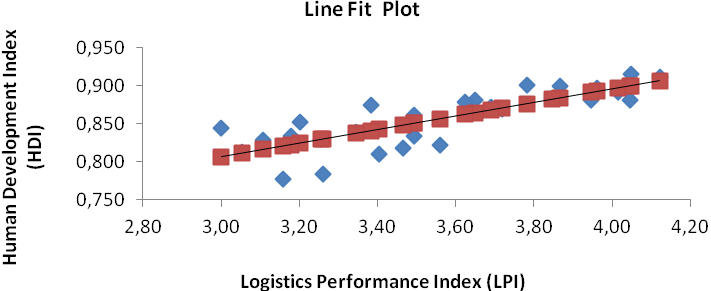
\includegraphics[width=0.8\textwidth]{figures/correlation_HDI_LPI.png}
    \caption{The correlation between the Logistics Performance Index (LPI) and the Human Development\cite{HDIvsLPI}}
    \label{fig:correlation_HDI_LPI}
\end{figure}


As shown in in figure \ref{fig:correlation_HDI_LPI} the relationship between European Union country 
logistics performance and quality of life is strong. However, transportation is also 
a net emmiter of \ce{CO2} in EU. According to the European Environment Agency (EEA) report domestic
transport is responsible for 29.17\% of total \ce{CO2} emissions in 2022\cite{EEA}. And yet the trend of 
domestic transport utilisation is still increasing.This is a clear indicator that transportation is sub-optimal and requires
 improvements in order to reduce the impact on environment. 

Public transport is seen a solution on how to tackle the problem of increasing \ce{CO2} emissions.
Efficient and reliable public transport systems can reduce the number of cars used, thus reducing 
the load on public roads and mitigating unnecessary accident risks. However, to acheive that
it there are some dificult challenges that need to be addressed. SOme of the most important aspects
that keep people in their car are:
    unreliable schedules,
    long waiting times,
    inconvenient routes,
    high ticket prices,
    overloaded buses

In the scope of this research some of the most important hurdles for public transport will be addressed.
The main focus of this paper will be put on increasing the efficiency of bus dispatching and scheduling.
By optimising the route and schedule, the number of buses utilised in the fleet can be reduced and 
the size of bus sent on route can be adjusted to the number of passengers expected. 
By doing so, the costs of operations should decrease thus, making public transportation services more
affordable and attractive to the society.

To optimise the dispatching and scheduling neural network models will be used. The models will
be trained on historical data on sales of tickets in bus stops. The developed model will be
used to predict the number of passengers in bus stops in the future. The decision on the size of the bus
to dispatch and stations to include in the route will be made by the dispatcher, but with real time
advice from the neural network model. 


\newpage
\section{Related work overview}

\hspace{1 em} The technologies for aggregating passenger flow data have had significant
advancements in the last decade. With the development of the Internet of Things (IoT)
devices, Intelligent Transport Systems (ITS) have become widely available for public
transportation fleet operators. Smart ticket composters, GPS tracking devices, automated
passenger counters (APC) and data transmission technologies such as 5G networks became
common with monitoring and managing public transport. 
The collected data can be used not only for tracking Key Performance Indicators (KPIs),
but also to model passenger flow and predict future demand. 

The passenger flow prediction could be divided in terms of prediction time scale: short-term
forecasting (minutes to hours), medium-term forecasting (hours to days) and long-term (months, seasons of the year).
For short term passenger flow forecasting, short term traffic flow forecasts have an effect. Moreover,
short term flow prediction could be divided in parametric and non-parametric models. Parametric models

Parametric models is the standard approach for short-term flow forecasting. Models such as 
Seasonal Autoregresive Integrated Moving Average (SARIMA) and Autoregressive Integrated Moving Average (ARIMA)
have been used to predict demands for fleet\cite{ARIMA}. These models are well suited for time series predictions
and widely used in the field of transportation management. However, due to linear nature of these models, they are not
well suited to capture the non-linear patterns in the data.

Non-parametric approach such as Long Short-Term Memory (LSTM) reccurent neural networks (RNN) have been used to predict passenger flow\cite{LSTM}.
However RNN models have a flaw of vanishing gradient problem, which makes it difficult to train the model for long sequences of data.
To overcome this problem, LSTM models were introduced. LSTM models have a memory cell that can store information for long periods of time.



\newpage
\begin{thebibliography}{99}
        \bibitem{HDIvsLPI}The Transport and Logistics Sector\’s Performance and the Social Development - A Comparison within the European Union - Scientific Figure on ResearchGate. Available from: correlation\_HDI\_LPI https://www.researchgate.net/figure/The-correlation-between-LPI-and-HDI-within-EU28-Source-of-data-World-Bank-United\_fig1\_275887205

        \bibitem{EEA}European Environment Agency. (2024). Greenhouse gas emissions from transport in Europe. Available from: \url{https://www.eea.europa.eu/data-and-maps/indicators/transport-emissions-of-greenhouse-gases/transport-emissions-of-greenhouse-gases-11}
        \bibitem{ARIMA}Chuwang, D.D.; Chen, W. Forecasting Daily and Weekly Passenger Demand for Urban Rail Transit Stations Based on a Time Series Model Approach. Forecasting 2022, 4, 904-924. https://doi.org/10.3390/forecast4040049
        \bibitem{LSTM} Shivaraj Halyal, Raviraj H. Mulangi, M.M. Harsha,
        Forecasting public transit passenger demand: With neural networks using APC data,
        Case Studies on Transport Policy,
        Volume 10, Issue 2,
        2022,
        Pages 965-975,
        ISSN 2213-624X,
        https://doi.org/10.1016/j.cstp.2022.03.011.
        (https://www.sciencedirect.com/science/article/pii/S2213624X22000633)
\end{thebibliography}
\end{document}
